
% \subsection{Useful Lemmas}
% \begin{lemma}[Fubini's theorem]
% \label{lem:fubini}
% Let $l:\Theta\times(\mathcal{X}\times\mathcal{Y})\rightarrow [0,\infty)$ satisfying Assumption~\ref{ass:loss}. Then for all $\mu\in\mathcal{M}^1_+(\Theta)$, $\int l(\theta,\cdot)d\mu(\theta)$ is Borel measurable; for  $\QQ\in\mathcal{M}^1_+(\mathcal{X}\times\mathcal{Y})$, $\int l(\cdot,(x,y))d\QQ(x,y)$ is Borel measurable. Moreover: $\int l(\theta,(x,y))d\mu(\theta)d\QQ(x,y)=\int l(\theta,(x,y))d\QQ(x,y)d\mu(\theta)$
% \end{lemma}

% \begin{lemma}
% \label{lem:usc1}
% Let $l:\Theta\times(\mathcal{X}\times\mathcal{Y})\rightarrow [0,\infty)$ satisfying Assumption~\ref{ass:loss}.
% Then for all $\mu\in\mathcal{M}^1_+(\Theta)$, $(x,y)\mapsto\int l(\theta,(x,y))d\mu(\theta)$ is upper semi-continuous and hence Borel measurable.  
% \end{lemma}
% \begin{proof}
% Let $(x_n,y_n)_n$ be a sequence of $\mathcal{X}\times\mathcal{Y}$ converging to $(x,y)\in\mathcal{X}\times\mathcal{Y}$.  For all $\theta\in\Theta$, $M-l(\theta,\cdot)$ is non negative and lower semi-continuous. Then by Fatou's Lemma applied:
% \begin{align*}
%   \int M-l(\theta,(x,y))d\mu(\theta)&\leq\int \liminf_{n\to\infty}  M-l(\theta,(x_n,y_n))d\mu(\theta)\\
%   &\leq  \liminf_{n\to\infty}  \int M-l(\theta,(x_n,y_n))d\mu(\theta) 
% \end{align*}

% Then we deduce that: $\int M- l(\theta,\cdot)d\mu(\theta)$ is lower semi-continuous and then $\int l(\theta,\cdot)d\mu(\theta)$ is upper-semi continuous.
% \end{proof}


% \begin{lemma}
% \label{lem:usc2}

% Let $l:\Theta\times(\mathcal{X}\times\mathcal{Y})\rightarrow [0,\infty)$ satisfying Assumption~\ref{ass:loss}
% Then for all $\mu\in\mathcal{M}^1_+(\Theta)$, $\QQ\mapsto\int l(\theta,(x,y))d\mu(\theta)d\QQ(x,y)$ is upper semi-continuous for weak topology of measures. 
% \end{lemma}
% \begin{proof}
%  $-\int l(\theta,\cdot)d\mu(\theta) $ is lower semi-continuous from Lemma~\ref{lem:usc1}. Then $M-\int l(\theta,\cdot)d\mu(\theta) $ is lower semi-continuous and non negative. Let denote $v$ this function. Let $(v_n)_n$ be a non-decreasing sequence of continuous bounded functions such that $v_n\to v$. Let $(\QQ_k)_k$ converging weakly towards $\QQ$. Then by monotone convergence:
 
%  \begin{align*}
%      \int vd\QQ = \lim_n \int v_nd\QQ =\lim_n \lim_k\int v_nd\QQ_k\leq \liminf_k \int vd\QQ_k
%  \end{align*}
%  Then $\QQ\mapsto\int vd\QQ$ is lower semi-continuous and then $\QQ\mapsto\int l(\theta,(x,y))d\mu(\theta)d\QQ(x,y)$ is upper semi-continuous for weak topology of measures. 
%  \end{proof}



% \begin{lemma}
% \label{lem:measure-sup}
% Let $l:\Theta\times(\mathcal{X}\times\mathcal{Y})\rightarrow [0,\infty)$ satisfying Assumption~\ref{ass:loss}.
% Then for all $\mu\in\mathcal{M}^1_+(\Theta)$, $(x,y)\mapsto \sup_{(x',y'),d(x,x')\leq\varepsilon,y=y'} \int l(\theta,(x',y'))d\mu(\theta)$ is universally measurable (i.e. measurable for all Borel probability measures). And hence the adversarial risk is well defined. 
% \end{lemma}
% \begin{proof}
% Let $\phi :(x,y)\mapsto \sup_{(x',y'),d(x,x')\leq\varepsilon,y=y'} \int l(\theta,(x',y'))d\mu(\theta)$. Then for $u\in\bar{\mathbb{R}}$:
% \begin{align*}
% \left\{\phi(x,y)>u\right\}=\text{Proj}_1\left\{((x,y),(x',y'))\mid\int l(\theta,(x',y'))d\mu(\theta)-c_\varepsilon((x,y),(x',y'))>u\right\}
% \end{align*}
% By Lemma~\ref{lem:usc2}: $((x,y),(x',y'))\mapsto \int l(\theta,(x',y'))d\mu(\theta)-c_\varepsilon((x,y),(x',y'))$ is upper-semicontinuous hence Borel measurable. So its level sets are Borel sets, and by~\citep[Proposition 7.39]{bertsekas2004stochastic}, the projection of a Borel set is analytic. And then $\left\{\phi(x,y)>u\right\}$ universally measurable thanks to~\citep[Corollary 7.42.1]{bertsekas2004stochastic}. We deduce that $\phi$ is universally measurable.
% \end{proof}



% \paragraph{Optimizer.} For each of our models, The optimizer we used in all our implementations is SGD with learning rate set to $0.4$ at epoch $0$ and is divided by $10$ at half training then by $10$ at the three quarters of training. The momentum is set to $0.9$ and the weight decay to $5\times10^{-4}$. The batch size is set to $1024$. 
% \paragraph{Adaptation of Attacks.} Since our classifier is randomized, we need to adapt the attack accordingly. To do so we used the expected loss:
% \begin{align*}
% \Tilde{l}\left((\bm{\lambda},\bm{\theta}),(x,y)\right) = \sum_{k=1}^L \lambda_k l(\theta_k,(x,y))
% \end{align*}
% to compute the gradient in the attacks, regardless the loss (DLR or cross-entropy). For the inner maximization at training time, we used a PGD attack on the cross-entropy loss with $\varepsilon=0.03$. For the final evaluation, we used the untargeted $DLR$ attack with default parameters.
% \paragraph{Regularization in Practice.} The entropic regularization in higher dimensional setting need to be adapted to be more likely to find adversaries. To do so, we computed PGD attacks with only $3$ iterations with $5$ different restarts instead of sampling uniformly $5$ points  in the $\ell_\infty$-ball. In our experiments in the main paper, we use a regularization parameter $\alpha=0.001$. The learning rate for the minimization on $\bm{\lambda}$ is always fixed to $0.001$. 
% \paragraph{Alternate Minimization Parameters.} Algorithm~\ref{algo:heuristic} implies an alternate minimization algorithm. We set the number of updates of $\bm{\theta}$ to $T_\theta = 50$ and, the update of $\bm{\lambda}$ to $T_\lambda = 25$. 

% \subsection{Effect of the Regularization}
% In this subsection, we experimentally investigate the effect of the regularization. In Figure~\ref{fig:xp-regularization}, we notice, that the regularization has the effect of stabilizing, reducing the variance and improving the level of the robust accuracy for adversarial training for mixtures (Algorithm~\ref{algo:heuristic}). The standard accuracy curves are very similar in both cases.


\begin{figure}[ht]
    \centering
    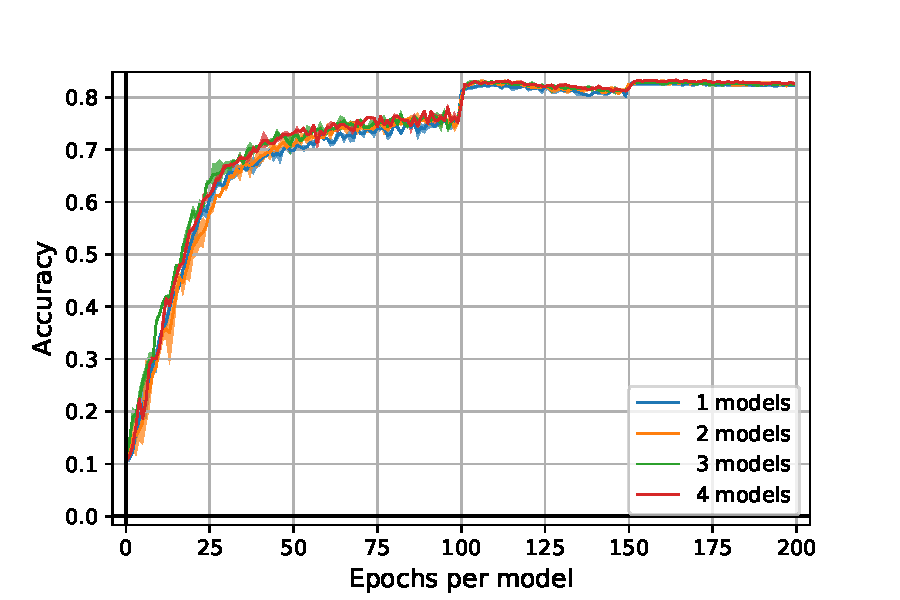
\includegraphics[width=0.40\textwidth]{Images/standard_acc_finalrun_ResNet18_1024_200_-1_bis.pdf}    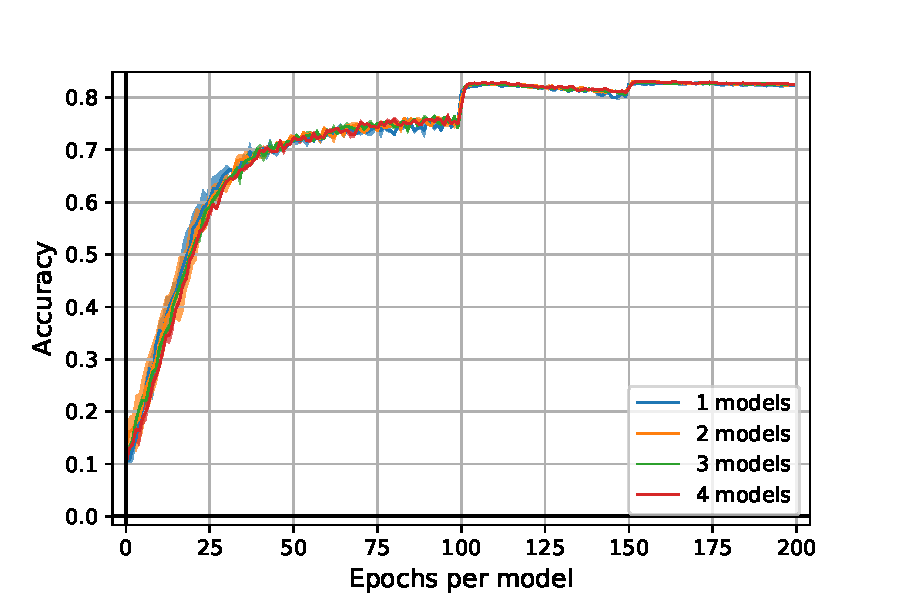
\includegraphics[width=0.40\textwidth]{Images/standard_acc_finalrun_ResNet18_1024_200_0.001_bis.pdf}\\

    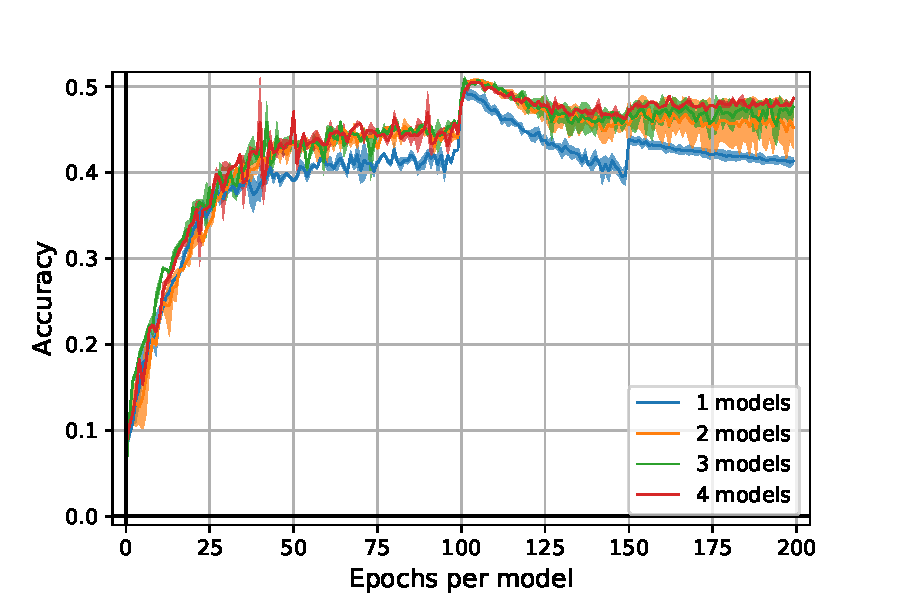
\includegraphics[width=0.40\textwidth]{Images/robust_acc_finalrun_ResNet18_1024_200_-1_bis.pdf}    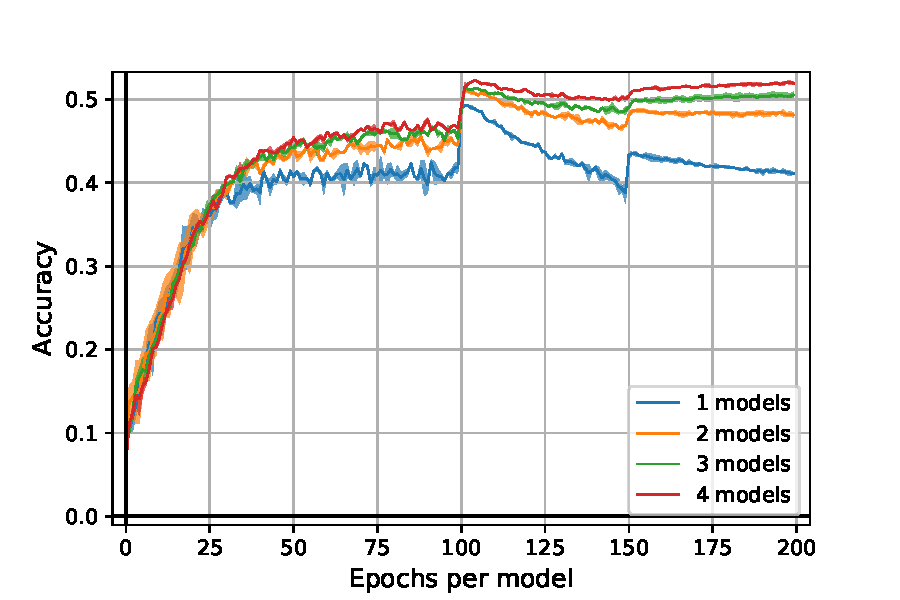
\includegraphics[width=0.40\textwidth]{Images/robust_acc_finalrun_ResNet18_1024_200_0.001_bis.pdf}
    \caption{On top: Standard accuracies over epochs with respectively no regularization and regularization set to $\alpha=0.001$. On bottom: Robust accuracies for the same parameters against PGD attack with $20$ iterations and $\varepsilon=0.03$.}
    \label{fig:xp-regularization}
\end{figure}

\subsection{Additional Experiments on WideResNet28x10}

We now evaluate our algorithm on WideResNet28x10~\cite{ZagoruykoK16} architecture. Due to computation costs, we limit ourselves to $1$ and $2$ models, with regularization parameter set to $0.001$ as in the paper experiments section. Results are reported in Figure~\ref{fig:xp-wideresnet}. We remark this architecture can lead to more robust models, corroborating the results from~\cite{gowal2020uncovering}.
\begin{figure*}[!ht]
\begin{center}

\begin{small}
\begin{tabular}{c|c|ccc} 
\textbf{ Models} & \textbf{Acc. }&\textbf{$\textrm{APGD}_\textrm{CE}$}& \textbf{$\textrm{APGD}_\textrm{DLR}$} & \textbf{Rob. Acc.} \\ \hline
 1 & $85.2\%$ &	$49.9\%$ & $50.2\%$ & $48.5\%$ \\ 
 2 & $\bm{86.0\%}$ & $\bm{51.5\%}$ & $\bm{52.1\%}$ & $\bm{49.6\%}$\\ 

\end{tabular}
\end{small}

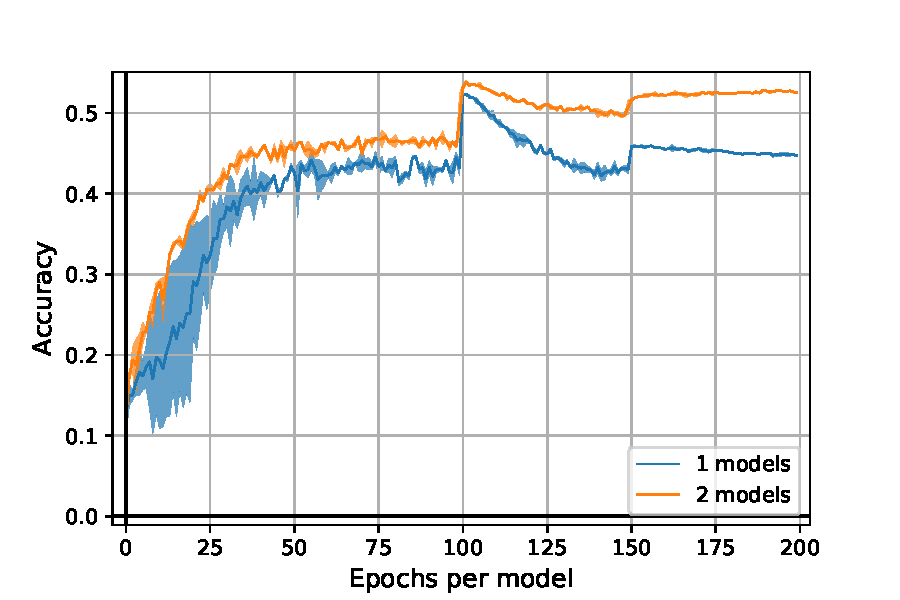
\includegraphics[width=0.35\textwidth]{Images/robust_acc_finalrun_WideResNet28x10_1024_200_0.001.pdf}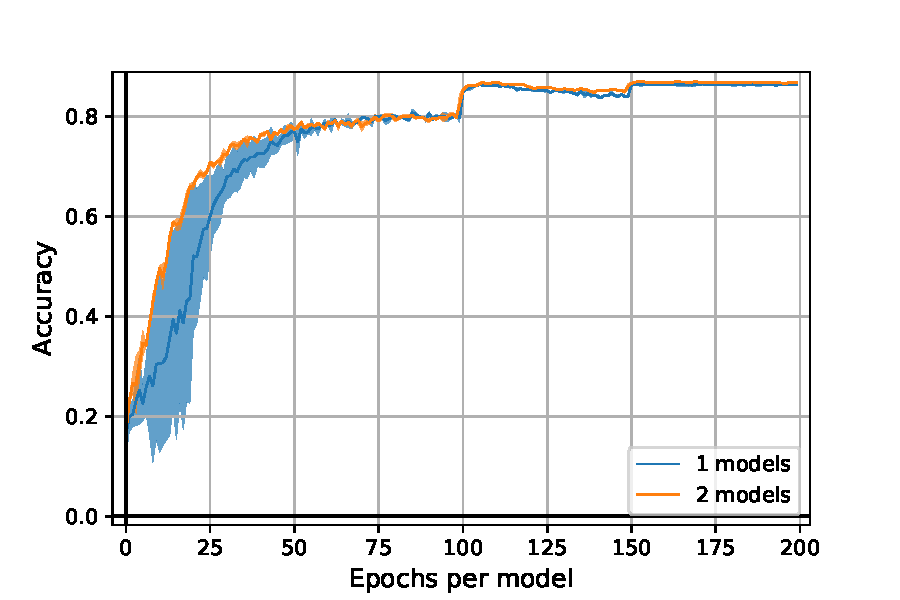
\includegraphics[width=0.35\textwidth]{Images/standard_acc_finalrun_WideResNet28x10_1024_200_0.001.pdf} 
  
\caption{Comparison of our algorithm with a standard adversarial training (one model) on WideResNet28x10. We reported the results for the model with the best robust accuracy obtained over two independent runs because adversarial training might be unstable. Standard and Robust accuracy (respectively in the middle and on right) on CIFAR-10 test images in function of the number of epochs per classifier with $1$ and $2$ WideResNet28x10 models. The performed attack is PGD with $20$ iterations and $\varepsilon=8/255$.}
\label{fig:xp-wideresnet}
\end{center}
\end{figure*}


\subsection{Overfitting in Adversarial Robustness}
We further investigate the overfitting of our heuristic algorithm. We plotted in Figure~\ref{fig:overfitting} the robust accuracy on ResNet18 with $1$ to $5$ models. The most robust mixture of $5$ models against PGD with $20$ iterations arrives at epoch $198$, \emph{i.e.} at the end of the training, contrary to $1$ to $4$ models, where the most robust mixture occurs around epoch $101$. However, the accuracy against AGPD with 100 iterations in lower than the one at epoch $101$ with global robust accuracy of $47.6\%$ at epoch $101$ and $45.3\%$ at epoch 198. This strange phenomenon would suggest that the more powerful the attacks are, the more the models are subject to overfitting. We leave this question to further works.


\begin{figure*}[!ht]
\begin{center}
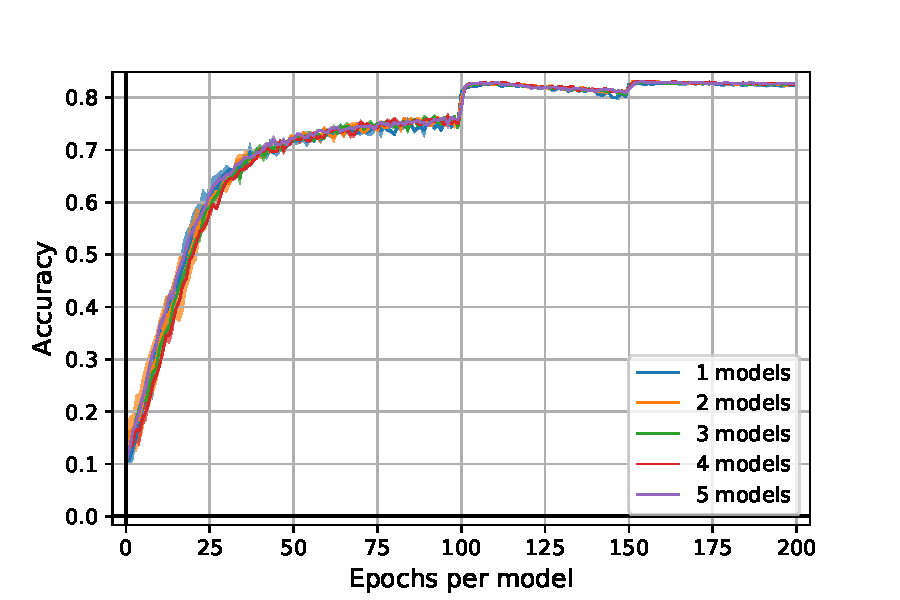
\includegraphics[width=0.49\textwidth]{Images/5_standard_acc_finalrun_ResNet18_1024_200_0.001.pdf}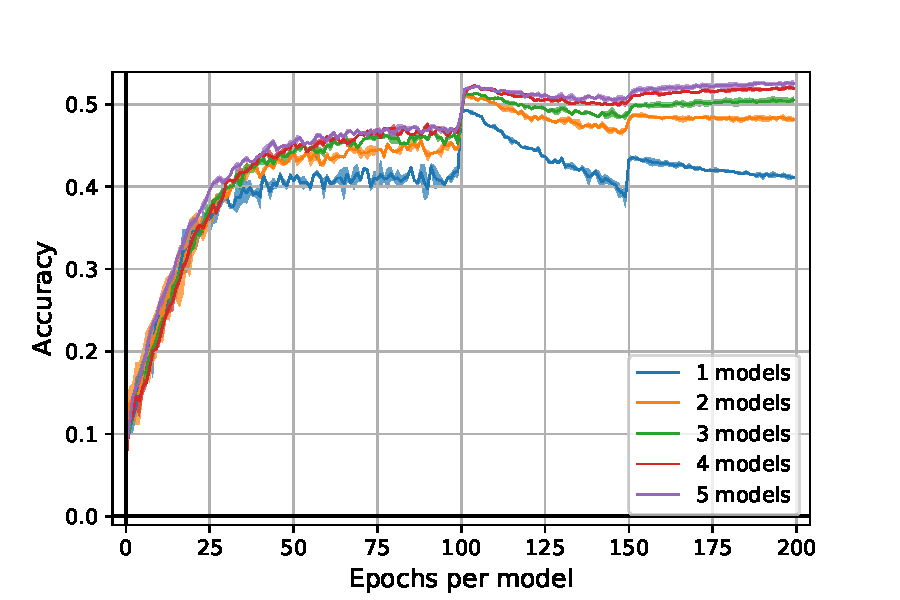
\includegraphics[width=0.49\textwidth]{Images/5_robust_acc_finalrun_ResNet18_1024_200_0.001.pdf} 

\caption{Standard and Robust accuracy (respectively on  left and on right) on CIFAR-10 test images in function of the number of epochs per classifier with $1$ to $5$ ResNet18 models. The performed attack is PGD with $20$ iterations and $\varepsilon=8/255$. The best mixture for $5$ models occurs at the end of training (epoch $198$).}
\label{fig:overfitting}
\end{center}
\end{figure*}



\section{Discussions and Open Questions}


\paragraph{On the need of Randomization.} While we give a concrete example where randomized is needed to be optimal in Section~\ref{sec:motiv-ex},~\citep{pydi2021many} show there is no duality gap when the classifier is allowed to play a deterministic measurable classifier. In other words, randomization would not be useful for this game. We conjecture, as the hypothesis class $\Theta$ grows, the duality gap decreases to $0$. However, in finite samples cases, it is not realistic to optimize over the space of measurable functions. One may ask if we could find conditions on the space of classifiers and the distribution $\PP$ such that randomization is required.~\citet{pinot2020randomization} partially answered this question when the attacker is regularized, but the general case is still an open question.

\paragraph{Statistical guarantees for randomized classifiers.} Although it is possible to derive uniform convergence bounds for the adversarial classification problem~\citep{yin2019rademacher,awasthi2020adversarial} for deterministic classifiers, deriving bounds for randomized classifiers is still an open question. One may think of adpating PAC-Bayes bounds~\citep{guedj2019primer} but the proof scheme cannot apply for adversarial classification. A first attempt to derive such bounds was proposed by~\citet{viallard2021pac}, but there is still much to do on this subject.


\paragraph{Learning Optimal Randomized Classifiers.} For a given loss, learning the optimal randomized classifier for a continuous parameter space is also an open question.  It is a difficult question since it requires learning over the space of ditributions. Attempts have been made to optimize over the space of distributions~\citep{chizat2021sparse,chizat2021convergence,kent2021frank} often using Wasserstein Gradient Flows~\citep{ambrosio2005gradient} and particular flows~\citep{wibisono2018sampling}. Recently,~\citet{domingo2020mean} proposed a particular flow to optimize a minmax problem in the space of distributions. While this paper gives good insights, the results are to preliminary to be adapted and applied to adversarial learning problems.
% \subsection{Additional Results}
% \label{sec:complements}
% \subsection{Equality of Standard Randomized and Deterministic Minimal Risks}
% \begin{prop}
% Let $\PP$ be a Borel probability distribution on $\mathcal{X}\times\mathcal{Y}$, and $l$ a loss satisfying Assumption~\ref{ass:loss}, then:
% \begin{align*}
%         \inf_{\mu\in\mathcal{M}^1_+(\Theta)} \risk(\mu) =\inf_{\theta\in\Theta} \risk(\theta)
% \end{align*}
% \end{prop}
% \begin{proof}
% It is clear that:         $\inf_{\mu\in\mathcal{M}^1_+(\Theta)} \risk(\mu) \leq \inf_{\theta\in\Theta} \risk(\theta)$. Now, let $\mu\in\mathcal{M}^1_+(\Theta)$, then:
% \begin{align*}
%     \risk(\mu)= \mathbb{E}_{\theta\sim\mu}(\risk(\theta))&\geq \essinf_\mu \mathbb{E}_{\theta\sim\mu} \left(\risk(\theta)\right)\\
%     &\geq\inf_{\theta\in\Theta} \risk(\theta).
% \end{align*}
% where $\essinf$ denotes the essential infimum.
% \end{proof}
% We can deduce an immediate corollary. 
% \begin{corollary}
% Under Assumption~\ref{ass:loss}, the dual for randomized and deterministic classifiers are equal.
% \end{corollary}

% \subsection{Decomposition of the Empirical Risk for Entropic Regularization}

% \begin{prop}
% Let $\hat{\PP}:=\frac1N\sum_{i=1}^N \delta_{(x_i,y_i)}$. Let $l$ be a loss satisfying Assumption~\ref{ass:loss}. Then we have:
% \begin{align*}
% \frac{1}{N}\sum_{i=1}^N\sup_{x,~d(x,x_i)\leq\varepsilon}\mathbb{E}_{\theta \sim \mu}\left[l(\theta,(x,y))\right]=\sum_{i=1}^N\sup_{\QQ_i\in\Gamma_{i,\varepsilon}}\mathbb{E}_{(x,y)\sim \QQ_i,\theta \sim \mu}\left[l(\theta,(x,y))\right]
% \end{align*}
% where $\Gamma_{i,\varepsilon}$ is defined as : 
% \begin{align*}
%     \Gamma_{i,\varepsilon}:=\Big\{\QQ_i\mid~\int d\QQ_i=\frac{1}{N},~\int c_{\varepsilon}((x_i,y_i),\cdot) d\QQ_i=0\Big\}.
% \end{align*}\end{prop}

% \begin{proof}
% This proposition is a direct application of Proposition~\ref{prop:dro_adv} for diracs $\delta_{(x_i,y_i)}$.
% \end{proof}

% % \subsection{On the NP-Hardness of Attacking a Mixture of Classifiers}
% % In general, the problem of finding a best response to a mixture of classifiers is in general NP-hard. Let us justify it on a mixture of linear classifiers in binary classification: $f_{\theta_k}(x) = \langle \theta,x\rangle$ for $k\in [L]$ and $\bm{\lambda}=\mathbf{1}_L/L$. Let us consider the $\ell_2$ norm and $x=0$ and $y=1$. Then the problem of attacking $x$ is the following:
% % \begin{align*}
% %     \sup_{\tau,~\lVert \tau\rVert\leq\varepsilon} \frac{1}{L}\sum_{k=1}^L\mathbf{1}_{\langle \theta_k,x+\tau\rangle\leq0}
% % \end{align*}
% % This problem is equivalent to a linear binary classification problem on $\tau$, which is known to be NP-hard.




% \subsection{Case of Separated Conditional Distribtions}
% \begin{prop} Let $\mathcal{Y} = \{-1,+1\}$. Let $\PP\in\mathcal{M}^1_+(\mathcal{X}\times\mathcal{Y})$. Let $\varepsilon>0$. For $i\in\mathcal{Y}$, let us denote $\PP_i$ the distribution of $\PP$ conditionally to $y=i$. Let us assume that  $d_\mathcal{X}(\supp(\PP_{1+1}),\supp(\PP_{-1}))>2\varepsilon$. Let us consider the nearest neighbor deterministic classifier : $f(x) =  d(x,\supp(\PP_{+1}))-d(x,\supp(\PP_{-1}))$ and the $0/1$ loss $l(f,(x,y))=\mathbf{1}_{yf(x)\leq 0}$. Then $f$ satisfies both optimal standard and adversarial risks: $\risk(f)=0$ and $\riskadv^\varepsilon(f)=0$.
% \end{prop}

% \begin{proof} Let 
% Let denote $p_i =\PP(y=i)$. Then we have
% \begin{align*}
%  \riskadv^\varepsilon(f)= p_{+1}\mathbb{E}_{\PP_{+1}}\left[\sup_{x',~d(x,x')\leq \varepsilon}\mathbf{1}_{ f(x')\leq 0}\right]+p_{-1}\mathbb{E}_{\PP_{-1}}\left[\sup_{x',~d(x,x')\leq \varepsilon}\mathbf{1}_{ f(x')\geq 0}\right]
% \end{align*}
% For $x\in \supp(\PP_{+1})$, we have, for all $x'$ such that $d(x,x')\neq 0$, $f(x')>0$, then: $\mathbb{E}_{\PP_{+1}}\left[\sup_{x',~d(x,x')\leq \varepsilon}\mathbf{1}_{ f(x')\leq 0}\right]=0$. Similarly, we have $\mathbb{E}_{\PP_{-1}}\left[\sup_{x',~d(x,x')\leq \varepsilon}\mathbf{1}_{ f(x')\geq 0}\right]=0$. We then deduce the result.
% \end{proof}
